\section{Decision Trees}

\begin{frame}{Decision Trees}
\begin{block}{Decision Tree}
    一个决策树是一个 Boolean Function $f: \mathbb{F}_2^{n} \to \mathbb{R}$ 的表示方法。它是一个含根二叉树,其中内部节点由某个$i \in [n]$来标记,每个内部节点的出边被标记为$0$或$1$,每个叶子节点都有一个实数值,且要求没有$i \in [n]$在一条从根到叶节点的路径上出现多于一次。
\end{block}
\begin{itemize}
    % \item 决策树是一个预测器$h: X \to Y$, 方法是从树的根节点一次访问每个孩子节点判断下一步走向,最终走到叶子节点。每个叶子节点对应一个$Y$中的元素。
    \item 称决策树的叶节点总个数为决策树的大小(size) $s$,称决策树根到叶节点路径的最大长度为决策树的深度(depth) $d$。
    \item 根据定义,每个决策树都对应一个有$n$个变量的布尔函数。
\end{itemize}
\end{frame}

\begin{frame}{Decision Trees Example}
    Example:
    \begin{center}
        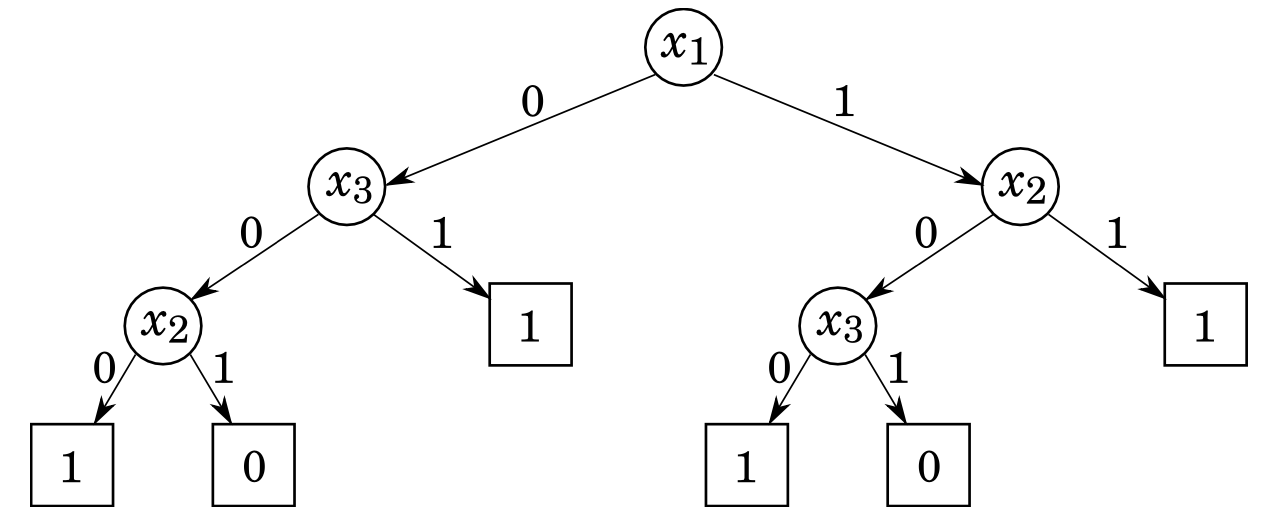
\includegraphics[width=0.65\textwidth]{assets/dtree.png}
    \end{center}

    Note: 这棵树事实上对应函数 $\text{Sort}_3$, 其中 $\text{Sort}_3(x_1, x_2, x_3) = 1$ 当且仅当 $x_1 \geqslant x_2 \geqslant x_3$ 或 $x_1 \leqslant x_2 \leqslant x_3$。
\end{frame}

\begin{frame}{Theoretical Guarantee}
    \begin{block}{Theorem: Convert decision tree to low degree sparse function}
        对任意有$s$个叶节点的决策树$T$,存在一个degree为$\log(s / \epsilon)$,$L_0$-norm(sparsity) 为 $s^{2} / \epsilon$ 的布尔函数 $h$ 能够 $4 \epsilon$-approximate $T$。 
    \end{block}
    证明思路:
    \begin{itemize}
        \item 将决策树$T$截断到深度为 $\log(s / \epsilon)$,最大误差为$\epsilon$。
        \item 截断后的树$T'$ 能用一个$L_1(f) \leqslant s, \text{deg}(f) = \log(s / \epsilon)$的布尔函数$f$ 严格表示。
        \item 上述满足$L_1(f) \leqslant s, \text{deg}(f) = \log(s / \epsilon)$的布尔函数$f$能用另一个满足$L_0(h) \leqslant s^{2} / \epsilon, \text{deg}(h) = \log (s / \epsilon)$的布尔函数$h$ 来 $\epsilon$-approximate 表示。
    \end{itemize}
    综上,$\left\| T-f \right\|^{2} \leqslant \epsilon$, $\left\| f-h \right\|^{2} \leqslant \epsilon$ 
    
    $\implies \left\| T - h \right\|^{2} \leqslant 2 \left\| T-f \right\|^{2} + 2 \left\| f-h \right\|^{2} \leqslant 4\epsilon$
\end{frame}

\begin{frame}{Practical Algorithms 1}
    由于使用上述定理提供的方法求low degree approximate function $h$的复杂度较高,实际中采用以下几种算法:
    \begin{itemize}
        \item LMN: 设$T$对应布尔函数$f$,均匀采样$m$个$f$ 定义域内的点$\left\{ x_i, i \in [m] \right\} $,计算 $f(x_i)$,对每个$|S| \leqslant \log(s / \epsilon)$的 $S$ 估计傅立叶系数$\hat{f}(S)\approx \frac{1}{m} \sum_{i=1}^{m} f(x_i) \chi _S(x_i)$。
        最后返回
        \[
            h = \sum_{S: |S| \leqslant \log(s / \epsilon)} \hat{f}(S) \chi _S
        \]
        \item Harmonica: 这个问题本质上是求一个在傅立叶基下稀疏的布尔函数,可以用compress sensing 范式求解。
    \end{itemize}
    \begin{center}
        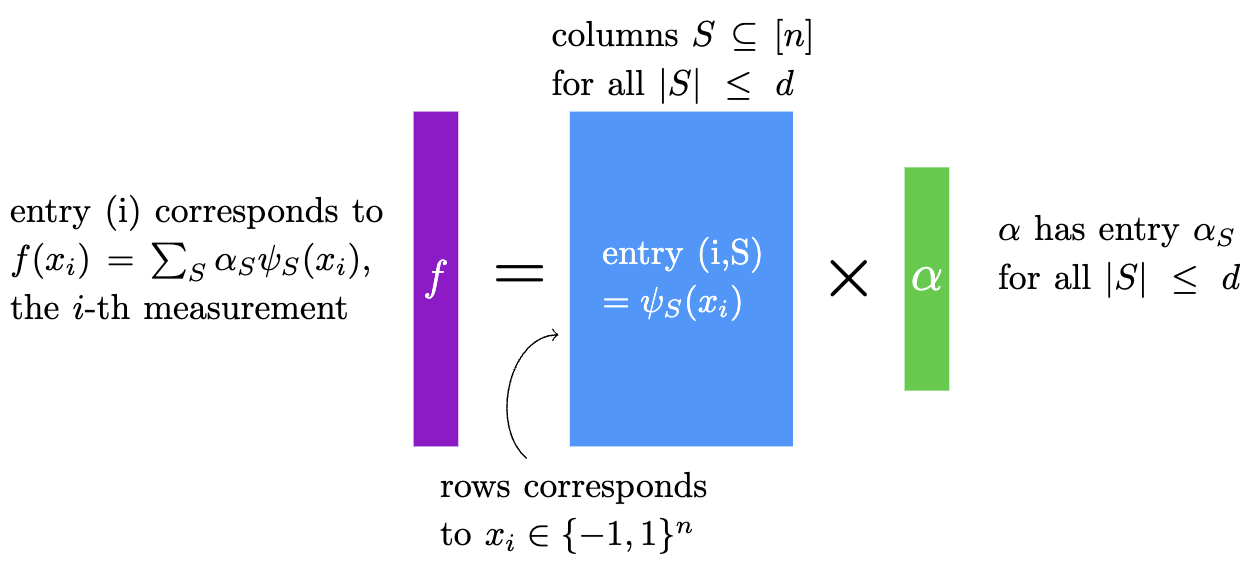
\includegraphics[width=0.4\textwidth]{assets/harmonica.png}
    \end{center}

\end{frame}

\begin{frame}{Practical Algorithms 2}
    现实问题中的决策树:给定若干样例,希望从样例中学习决策树。

    Example:
    \begin{center}
        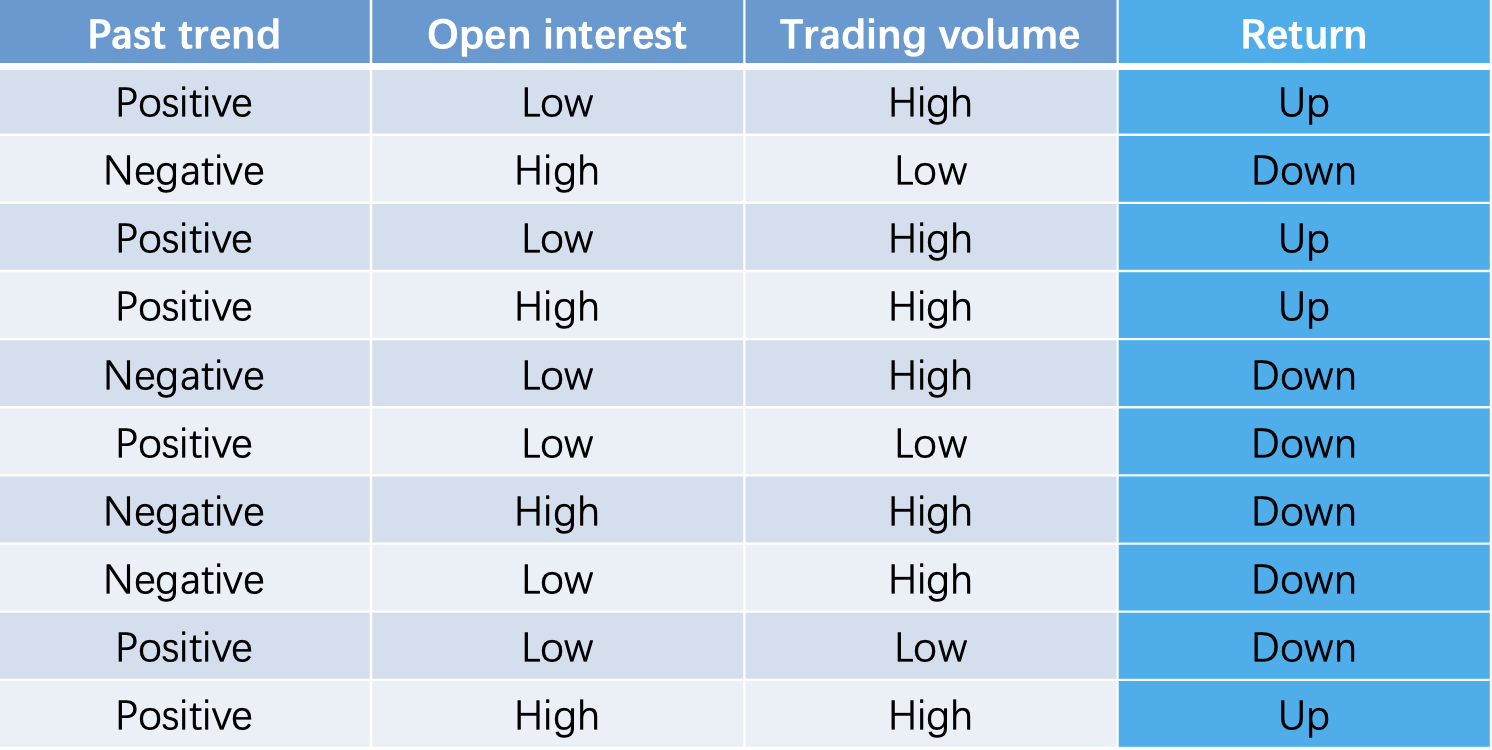
\includegraphics[width=0.65\textwidth]{assets/learndte.png}
    \end{center}

\end{frame}

\begin{frame}{Practical Algorithms 2}
    与上面的approach不同,另一种方法是递归选取最重要的变量作为内部节点划分样例。

    算法:
    \begin{center}
        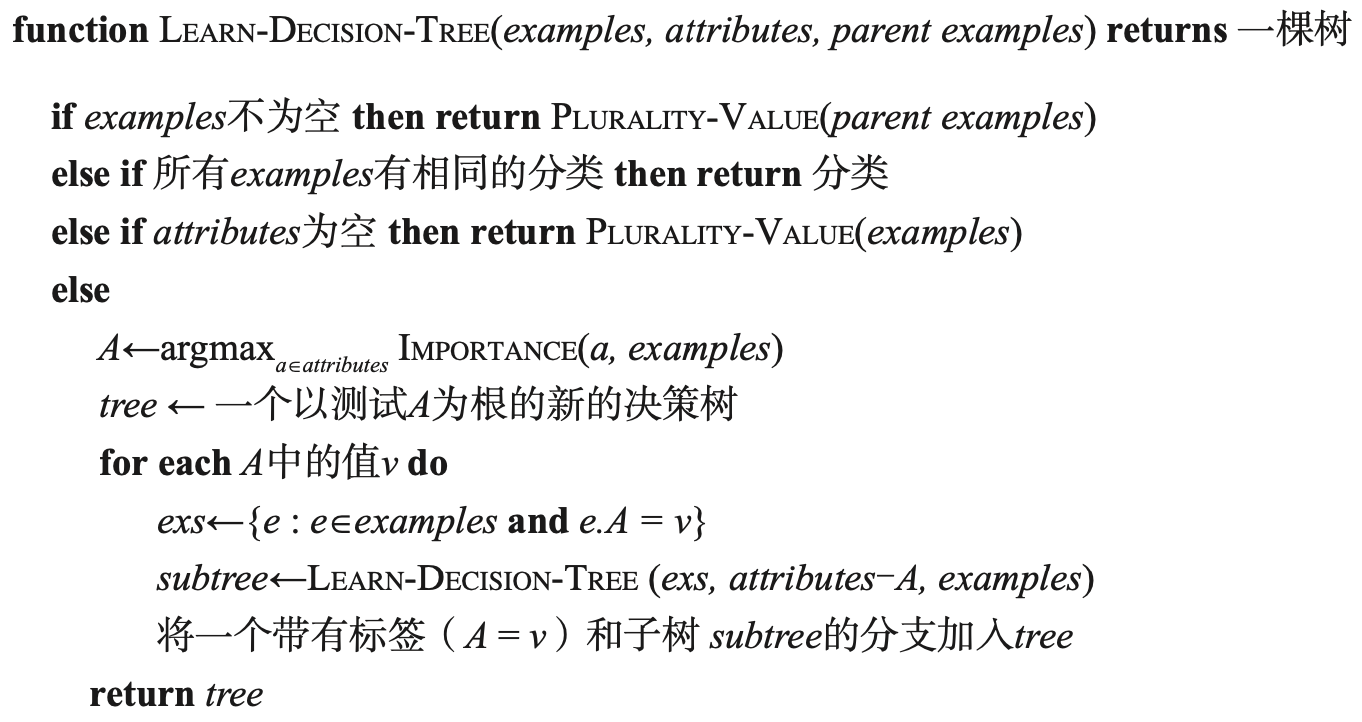
\includegraphics[width=0.6\textwidth]{assets/learndta.png}
    \end{center}
    解释:每次根据某种准则选择最重要的变量$i$(若某变量的取值几乎决定了最终的类别是什么,说明这个变量较重要)

\end{frame}

\begin{frame}{Gini Index}
    \begin{itemize}
        \item Gini Index 是一种判断某个变量是否重要的一种准则。
        \item 定义:对变量A,$\text{Gini}(A)= \sum_{a} p(A=a) \text{Gini}(a)$, 其中$\text{Gini}(a) = 1- \sum_{i}p_i^{2}$(详见课件例子)
        \item $\text{Gini}(a)$ 越小表示区分度越好(如果一个变量$A$取正时所有结果都是正,一个变量取负时所有结果都是负,则$\text{Gini}(A) = 0$),故每次划分变量时选择$\text{Gini}(A)$最小的变量$A$。
        \item 其他准则:Information Gain
    \end{itemize}
\end{frame}
